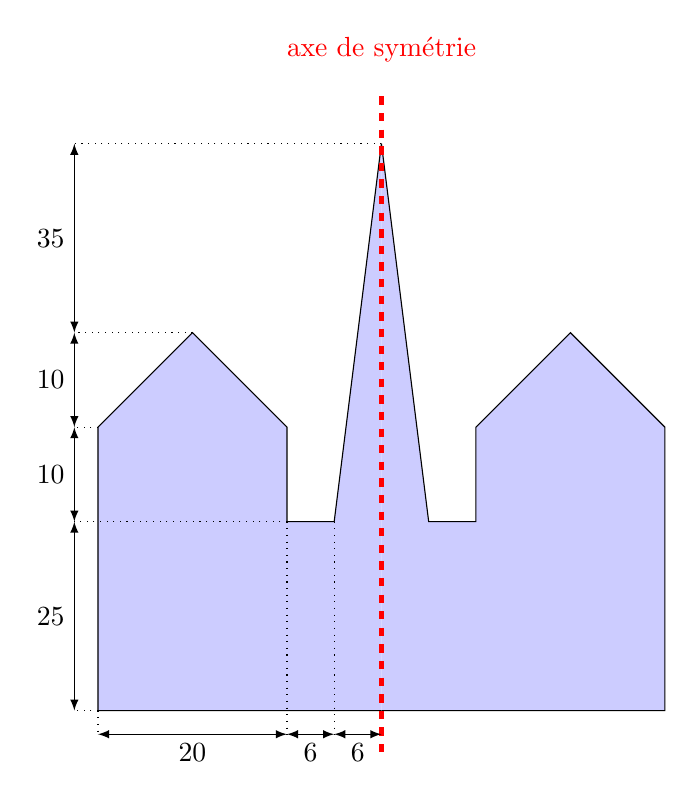
\begin{tikzpicture}[scale=0.6]
    \draw[fill=blue!20] (0,3) -- (1,-5) -- (2,-5) -- (2,-3) -- (4,-1) -- (6,-3) -- (6,-9) -- (0,-9) ;  
    \draw[fill=blue!20] (0,3) -- (-1,-5) -- (-2,-5) -- (-2,-3) -- (-4,-1) -- (-6,-3) -- (-6,-9) -- (0,-9) ;
    \draw[dashed, color=red, ultra thick] (0,4) -- (0,-10) ;
    \node[color=red] at (0,5) {axe de symétrie} ;
    \draw[dotted] (0,3) -- (-6.5,3) ;
    \draw[dotted] (-4,-1) -- (-6.5,-1) ;
    \draw[dotted] (-6,-3) -- (-6.5,-3) ;
    \draw[dotted] (-2,-5) -- (-6.5,-5) ;
    \draw[dotted] (-6,-9) -- (-6.5,-9) ;
    \draw[<->,>=latex] (-6.5,-1) -- (-6.5,3) node[midway, left]{$35$};
    \draw[<->,>=latex] (-6.5,-3) -- (-6.5,-1) node[midway, left]{$10$};
    \draw[<->,>=latex] (-6.5,-5) -- (-6.5,-3) node[midway, left]{$10$};
    \draw[<->,>=latex] (-6.5,-9) -- (-6.5,-5) node[midway, left]{$25$};
    \draw[dotted] (-6,-9) -- (-6,-9.5) ;
    \draw[dotted] (-2,-5) -- (-2,-9.5) ;
    \draw[dotted] (-1,-5) -- (-1,-9.5) ;
    \draw[<->,>=latex] (-6,-9.5) -- (-2,-9.5) node[midway, below]{$20$};
    \draw[<->,>=latex] (-2,-9.5) -- (-1,-9.5) node[midway, below]{$6$};
    \draw[<->,>=latex] (-1,-9.5) -- (0,-9.5) node[midway, below]{$6$};
\end{tikzpicture}